\documentclass[11pt]{article}
%\usepackage{fullpage,graphicx,algorithm,algorithmic,bm,amsmath,amsthm,amssymb,color,hyperref,cite,natbib}

% if you need to pass options to natbib, use, e.g.:
%\PassOptionsToPackage{numbers}{natbib}
\usepackage{natbib,fullpage}
\usepackage{bm,amsmath,amsthm,amssymb,multicol,algorithmic,algorithm,enumitem}
\usepackage{wrapfig,lipsum}
\usepackage[textwidth=1cm,textsize=footnotesize]{todonotes}

% ready for submission
\usepackage{neurips_2019}

\usepackage[colorlinks=true,
linkcolor=red,
urlcolor=blue,
citecolor=blue]{hyperref}
\usepackage{hyperref}
\usepackage{cleveref}

\setlength{\parskip}{.2cm}

\newtheorem{Fact}{Fact}
\newtheorem{Lemma}{Lemma}
\newtheorem{Prop}{Proposition}
\newtheorem{Theorem}{Theorem}
\newtheorem{Def}{Definition}
\newtheorem{Corollary}{Corollary}
\newtheorem{Conjecture}{Conjecture}
\newtheorem{Property}{Property}
\newtheorem{Observation}{Observation}
%\theorembodyfont{\rmfamily}
\newtheorem{Exa}{Example}
\newtheorem{assumption}{H\!\!}
\newtheorem{assumptionA}{S\!\!}
\newtheorem{Remark}{Remark}

%%%%%%%%%%% Stuffs for Tikz %%%%%%%%%%%%%%%%%%
\usepackage{pgfplots}
\usepackage{xargs}
\usepackage{stmaryrd}
\usetikzlibrary{arrows,shapes,calc,tikzmark,backgrounds,matrix,decorations.markings}
\usepgfplotslibrary{fillbetween}

\pgfplotsset{compat=1.3}

\usepackage{relsize}
\tikzset{fontscale/.style = {font=\relsize{#1}}
    }

\definecolor{lavander}{cmyk}{0,0.48,0,0}
\definecolor{violet}{cmyk}{0.79,0.88,0,0}
\definecolor{burntorange}{cmyk}{0,0.52,1,0}

\def\lav{lavander!90}
\def\oran{orange!30}

\definecolor{asuorange}{rgb}{1,0.699,0.0625}
\definecolor{asured}{rgb}{0.598,0,0.199}
\definecolor{asuborder}{rgb}{0.953,0.484,0}
\definecolor{asugrey}{rgb}{0.309,0.332,0.340}
\definecolor{asublue}{rgb}{0,0.555,0.836}
\definecolor{asugold}{rgb}{1,0.777,0.008}

%%%%%%%%%%%%%%%%%%%%%%%%%%%%%%%%%%%%%


\usepackage{shortcuts_OPT}

%\renewcommand{\textwidth}{5.5in}

% Here's the definition of Sb, stolen from amstex
    \makeatletter
    \def\multilimits@{\bgroup
  \Let@
  \restore@math@cr
  \default@tag
 \baselineskip\fontdimen10 \scriptfont\tw@
 \advance\baselineskip\fontdimen12 \scriptfont\tw@
 \lineskip\thr@@\fontdimen8 \scriptfont\thr@@
 \lineskiplimit\lineskip
 \vbox\bgroup\ialign\bgroup\hfil$\m@th\scriptstyle{##}$\hfil\crcr}
    \def\Sb{_\multilimits@}
    \def\endSb{\crcr\egroup\egroup\egroup}
\makeatother

\newtheoremstyle{t}         %name
    {\baselineskip}{2\topsep}      %space above and below
    {\rm}                   %Body font
    {0pt}{\bfseries}  %Heading indent and font
    {}                      %after heading
    { }                      %head after space
    {\thmname{#1}\thmnumber{#2}.}

\theoremstyle{t}
\newtheorem{q}{Q}
\parindent=0pt

%\newcommand{\eric}[1]{\todo[color=red!20]{{\bf EM:} #1}}
%\newcommand{\erici}[1]{\todo[color=red!20,inline]{{\bf EM:} #1}}
%\newcommand{\belhal}[1]{\todo[color=green!20]{{\bf BK:} #1}}
%\newcommand{\belhali}[1]{\todo[color=green!20,inline]{{\bf BK:} #1}}
%\newcommand{\toco}[1]{\todo[color=yellow!20]{{\bf To:} #1}}



\makeatletter
\DeclareRobustCommand*\cal{\@fontswitch\relax\mathcal}
\makeatother

\begin{document}
\title{Variational Inference and Dropout}
%\author{}
\date{\today}

\maketitle

\begin{abstract}

\end{abstract}

\section{Variational Inference for Latent Variable Model} Let $x = (x_i,  i \in \inter)$ and $y = (y_i,  i \in \inter)$ be i.i.d. input-output pairs and $w \in \Wset[] \subseteq \rset^J$ be a latent variable. The joint distribution of $y,w$ can be written as:
\begin{equation} \textstyle
    p(y,w | x) = p(w)\prod_{i=1}^{n}{p_i(y_i | x_i, w)}
\end{equation}
Our goal is to compute the posterior distribution $p(w|y,x)$ given the input-output pairs $x$, $y$. 
%Define the Kullback Leibler (KL) divergence for any two distributions $q(\cdot)$ and $p(\cdot)$ defined on $\Wset[]$ as
%\beq
%\infdiv{ q(w) }{ p(w) } \eqdef \int_{\Wset[]} q(w) \log \frac{ q(w) }{ p(w) }~\dw \eqsp.
%\eeq
The variational Inference (VI) algorithm \citep{blei2017vi} consists of minimizing the KL divergence between a candidate family of parametric distributions $\{q(w, \param ), \param \in \Param \}$ and the posterior distribution $p(w|y,x)$ of the global latent variable $w$. For example, $q(w; \param )$ belongs to a simple family of distributions such as the multivariate Gaussian family with mean $\rho$ and covariance matrix $\sigma^2 \Id$, where we have $\param = (\rho, \sigma^2) \in \Param = \mathbb{R}\times \mathbb{R}^{*}_{+}$.
VI can be framed as an optimization problem, usually in terms of KL divergence, of the following form:
\begin{equation} \label{eq:VI}
\param^*  = \argmin_{ \param \in \Param }~\infdiv{q(w; \param )}{p(w|y,x)} = \argmin_{\param \in \Param } ~{\cal L}(\param )
\end{equation}
where ${\cal L}(\param) \eqdef n^{-1} \sum_{i=1}^{n}{{\cal L}_i(\param)}$ for $\param \in \Param$ with :
\begin{equation}\label{eq:variationalobjective}
{\cal L}_i(\param) \eqdef -\int_{\Wset[]}{q(w;\param) \log p_i(y_i | x_i, w) \dw}+ \frac{1}{n} \infdiv{q(w;\param)}{p(w)} = r_i(\param) + d(\param),
\end{equation}
%Even though this procedure makes inference analytical for a large class of models, it still lacks in many ways.
%This technique
Directly optimizing the finite sum objective \eqref{eq:VI} can be infeasible especially when $n \gg 1$. This is because evaluating the objective function ${\cal L}( \param )$ requires a full pass of computation over the entire dataset, and this approach does not adapt to complex models when the last integral cannot be evaluated analytically. For instance, such optimization problem is notoriously hard for Bayesian neural networks \citep{neal1996bnn}.

To apply the MISSO method with a stochastic surrogate model \eqref{eq:integralsurrogate}, we consider the following quadratic surrogate function. For any $i \in \inter$, we take:
\begin{equation}
\sur{i}{\param}{\op} \eqdef {\cal L}_i(\op) + \pscal{ \nabla {\cal L}_i(\op)} { \param - \op} +\frac{L}{2}\|\op -\param \|^2
\end{equation}
where $L$ is the smoothness modulus of ${\cal L}_i$ at $\op$.
To compute the gradient $\nabla {\cal L}_i(\op)$, we apply the re-parametrization technique suggested in \citep{paisley2013,kingma, blundell2015weight}.
Let $t: \Param \times \rset^d \mapsto \rset^d$ be a measurable function and $\phi$ be the density of the standard normal distribution $\mathcal{N}_d(0,\Id)$. The function $t$ is designed such that for all $\op \in \Param$ and for $\epsilon \sim \phi(\cdot)$, the distribution of the random vector $W = t(  \op, \epsilon  )$ is the same as $q(\cdot, \op )$. It follows from \citep[Proposition~1]{blundell2015weight} that:
\beq
\nabla \int_{\Wset[]}{\log p_i(y_i| x_i, w)q(w, \op)\dw} =  \int_{\rset^d}{\jacob{t}{\param}{ \op ; e}  \nabla \log p_i(y_i | x_i, t(  \op, e ) )\phi(e)\mathrm{d}e}
\eeq
where for each $e \in \mathbb{R}^d$, $\jacob{t}{\param}{ \op; e}$ is the Jacobian of the function $t(\cdot,e)$ with respect to $\param$ evaluated at $\op$.  Consequently, we can apply the MISSO method to tackle the VI problem with the pair $\left(\rsur{i}{\param}{\op}{e}, \phi(e)\right)$ where $\rsur{i}{\param}{\op}{e}$ reads:
\begin{align}\label{pairvi}
\rsur{i}{\param}{\op}{e} \eqdef & \left( - \log p_i(y_i | x_i, t( \op,e)) +  d(\op) \right) \nonumber \\
& + \left(- \jacob{t}{\param}{ \op ; e}\nabla \log p_i(y_i | x_i, t(\op,e))+ \grd d(\op)\right)^\top (\param - \op )+\frac{L}{2}\| \param - \op\|^2
\end{align}



\section{Numerical Experiments} \label{sec:numerical}

\subsection{Fitting Bayesian LeNet-5 on MNIST:}
In this experiment, we implement the MISSO algorithm for variational inference in the Bayesian variant of LeNet-5 \citep{lecun1998gradient} (architecture is described in Appendix~\ref{appendix:bnn}).
We train this network on the MNIST dataset \citep{lecun1998mnist} used extensively as a benchmark example. The training set is composed of $N=55\,000$ handwritten digits, $28 \times 28$ images. Each image is labelled with its corresponding number (from zero to nine).

Given weight matrices $(w_\ell)_{\ell=1}^L \in \Wset[]^L$, we put, for each layer $\ell$ a standard Gaussian prior distributions over those weights: $p(w_\ell) = \mathcal{N}(0,I)$, as in \citep{gal2015bayesian}.
We denote by $f(x_i,(w_\ell)_{\ell=1}^L)$ the output of the nested function describing the neural network with weights $(w_\ell)_{\ell=1}^L \in \Wset[]^L$ taking as input a data sample $x_i$.
We assume a softmax likelihood in that classification task: $p(y_i|x_i,w) = \textrm{Softmax}(f(x_i,(w_\ell)_{\ell=1}^L))$.

The variational distribution $q(w,\theta)$ belongs to the Gaussian multivariate distribution family.
Here, the MISSO algorithm coincides with a mini-batch version of the Variational Inference algorithm. At iteration $k$, minimizing the sum of stochastic surrogates defined as in \eqref{eq:ssur} and by the quantities \eqref{pairvi} yields the following MISSO update: pick a function index $I_k$ uniformly on $\inter$, sample a Monte Carlo batch $ \{ e_{m}^{(k)} \}_{m=1}^{\Bsize{k}}$ from the standard Gaussian distribution and update the parameters as $\hp{k} = \frac{1}{n}\sum_{i=1}^{n}{\hp{\tau_{i}^{k}}} - \frac{1}{2 \gamma} \sum_{i=1}^{n}{\hat{{\bm{m}}}^k_i}$ where $\hat{{\bm{m}}}^k_i$ are defined recursively as follows:
\begin{align}\label{missoupdate}
 \hat{{\bm{m}}}^{(k)}_i &\triangleq
  \begin{cases}
  - \frac{1}{\Bsize{k}}\sum_{m=0}^{\Bsize{k}-1}{ \jacob{\param}{t}{e_{m}^{(k)}}\nabla_{\param} \log p_i(y_i,x_i|t(\param,e_{m}^{(k)}))} + \nabla d(\hp{k-1})     & \text{if } i \in I_k \\
  \hat{{\bm{m}}}^{(k-1)}_{i}         & \text{otherwise}
  \end{cases}
\end{align}

%\begin{enumerate}
%    \item Pick a function index $I_k$ uniformly on $\inter$.
%    \item Sample a Monte Carlo batch $ \{ e_{m}^{(k)} \}_{m=1}^{\Bsize{k}}$ from the standard Gaussian distribution.
%    \item Set $\hp{k} = \frac{1}{n}\sum_{i=1}^{n}{\hp{\tau_{i}^{k}}} - \frac{1}{2 \gamma} \sum_{i=1}^{n}{\hat{{\bm{m}}}^k_i}$ where $\hat{{\bm{m}}}^k_i$ are defined recursively as follows:
%\begin{align}\label{missoupdate}
% \hat{{\bm{m}}}^{(k)}_i &\triangleq
%  \begin{cases}
%  - \frac{1}{\Bsize{k}}\sum_{m=0}^{\Bsize{k}-1}{ \jacob{\param}{t}{e_{m}^{(k)}}\nabla_{\param} \log p_i(y_i,x_i|t(\param,e_{m}^{(k)}))} + \nabla d(\hp{k-1})     & \text{if } i \in I_k \\
%  \hat{{\bm{m}}}^{(k-1)}_{i}         & \text{otherwise}
%  \end{cases}
%\end{align}
%\end{enumerate}


We compare the convergence behaviors of the following state of the art optimization algorithms, using their vanilla implementations on TensorFlow \citep{tensorflow2015-whitepaper}: the ADAM \citep{kingma:adam}, the Momentum \citep{sutskever2013mom} the \textit{Bayes by Back-prop} (BBB) \citep{blundell2015weight} and the Dropout \citep{hinton2012dropout} algorithms versus our MISSO update.
The loss function \eqref{eq:variationalobjective} and its gradients were computed by Monte Carlo integration using Tensorflow Probability library, based on the reparametrization trick.
We use the following hyperparameters for all runs: the learning rate is set to $10^{-3}$, we run $100$ epochs and use a mini-batch size of $128$.\vspace{-.2cm}



\begin{figure}[H]
  \centering
    % \includegraphics[width=\textwidth]{pic_paper/bnn5.png}
    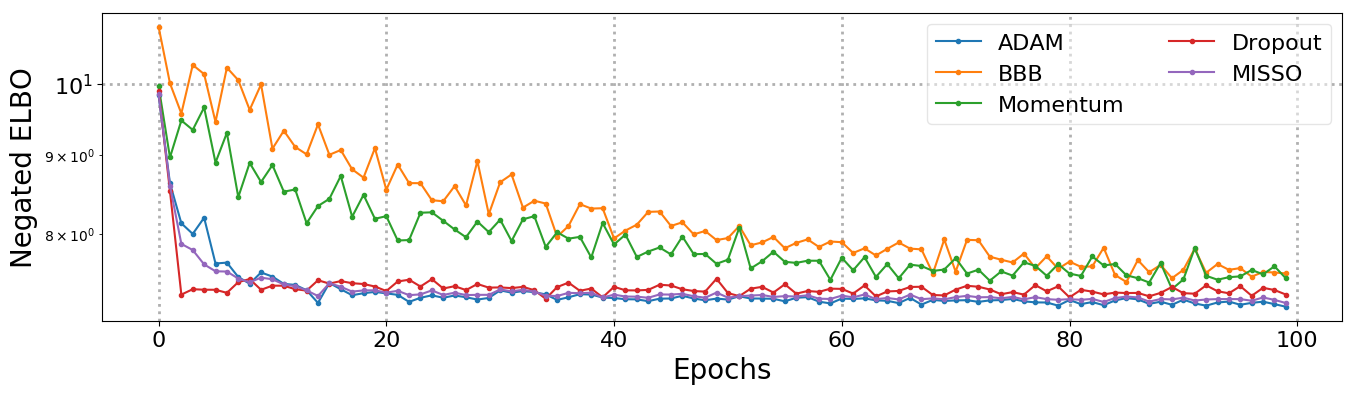
\includegraphics[width=.9\textwidth]{pic_paper/bnn2.png}\vspace{-.2cm}
  \caption{(Incremental Variational Inference) Convergence of the negated ELBO on MNIST.}
  \label{fig:misso}
\end{figure}

%We assume that there exists $L_{\sf r} < \infty$ such that
%\beq
%| \rsur{i}{\param}{\op}{z_i} - \rsur{i}{\param'}{\op}{z_i} | \leq L_{\sf r} \| \param - \param' \|,~~
%| \rsur{i}{\param}{\op}{z_i} - \rsur{i}{\param}{\op'}{z_i} | \leq L_{\sf r} \| \op - \op' \|,
%\eeq
%for any $\param,\param',\op,\op' \in \Param^4$.

\bibliographystyle{abbrvnat}
\bibliography{ref}

\newpage

\appendix

 \subsection{Incremental Variational Inference for MNIST}
 \subsubsection{Bayesian LeNet-5 Architecture}\label{appendix:bnn}


\begin{table}[h]
\begin{center}
    \label{table:lenet}
\begin{tabular}{ l c c c c r}
  \hline
  layer type & width & stride& padding & input shape& nonlinearity \\
  \hline
convolution ($5 \times 5$) & 6 & 1 & 0 & $1 \times 32 \times 32$ & ReLU \\
max-pooling ($2 \times 2$) &  & 2 & 0 & $6 \times 28 \times 28$ & \\
convolution ($5 \times 5$) & 6 & 1 & 0 & $1 \times 14 \times 14$ & ReLU \\
max-pooling ($2 \times 2$) &  & 2 & 0 & $16 \times 10 \times 10$ & \\
fully-connected & 120 &  &  & $400$ & ReLU \\
fully-connected & 84 &  &  & $ 120$ & ReLU \\
fully-connected & 10 &  &  & $ 84$ &  \\
  \hline
\end{tabular}
    \caption{LeNet-5 architecture}
\end{center}
\end{table}

%\linespread{1.1}
%\normalsize





%-----------------------------------------------------------------------------
%\vspace{0.4cm}

\end{document}
